\chapter{Background}
\label{chap:background}

For a set of robot to operate correctly, a vast infrastructure of software is generally required. Developing this directly without the use of any frameworks or libraries would require a large amount of person hours, in terms of both design and implementation time. Many different subsystems are required, each of which would require a deep technical understanding of the underlying intricacies. Typical systems require a means for communicating with hardware, locomotion control for movement, vision systems for guidance and environment mapping, autonomous navigation, means of user interaction, and so on. The complexity of each of these is such that they are research fields in their own right. 

However, through the use of ROS it is possible to gain access to these state-of-the-art functionalities free of charge, both in terms of cost in person hours. The open-source nature of ROS is such that any innovations made by other developers can be easily shared to the rest of the community. This offloads the complex understanding to smaller development teams which have expertise in that particular area.

The following sections in this chapter elaborate on the features of the ROS and our robot hardware, explaining why they are relevant to this project. This will provide a basis of understanding necessary for the implementation chapter and beyond.

%%%%%%%%%%%%%%%%%%%%%%%%%%%%%%%%%%%%%%%%%%%%%%%%%%%%%%%%%%%%%%%%%%%%%%%%%%%%%%%%%%%%%%%%%%%%%%%%%%%%

\section{Robot Operating System}

The \emph{Robot Operating System} (ROS) is an open-source framework for creating robot control systems, developed by \emph{Willow Garage} \cite{ros_paper}. ROS can be primarily thought of as a message-passing framework. A number of discrete processes, perhaps some even on a remote machine, communicate through a single broker service (the ROS "master") using an XMLRPC-based API. Each process performs a small part of a larger task, sharing data with other nodes through common data types.

ROS functions as a distributed system by default. Specifically, the processes can run on a machine different from that of the broker. The processes can then connect to the broker over a network, receiving data seamlessly from any other processes in the system. In cases where nodes are running on the same machine as the broker, they are simply connecting to the local machine. This can be used to offload complex computations onto another machine as necessary. To give an example, an embedded system on a robot running ROS can be collecting sensor data and issues hardware commands. This embedded system can then be communicating to a more powerful machine, acting as a base station. This base station can perform the more complex operations such as sensor data interpretation and path planning, relaying the commands back to the embedded system to be carried out.

\subsection{Supported Platforms}
At the time of writing, the latest version of ROS is \emph{Hydro Medusa} which primarily targets the \emph{Ubuntu} Linux distrubution, specifically versions 12.04 (LTS) to 13.04 \cite{ros_wiki_installation, ros_wiki_installation_ubuntu}. An Ubuntu repository containing binaries for ROS and its standard library of packages is available allowing for a trivial installation process, as well as allowing any updates to be delivered and installed with simplicity.

Experimental support is also available for other Linux distributions and systems, such as Ubuntu ARM, OS X, Debian, Arch Linux, Windows, and a number of embedded platforms \cite{ros_wiki_installation}. As the source code for ROS is freely available, it is possible to compile it on any system as long as the relevant supporting libraries are available.

\subsection{Nodes}
In ROS terminology, a processes is referred to as a \emph{node}. A node is simply a process that is connected to the ROS broker, performing some sort computation \cite{ros_paper}.

Nodes need not be tied to any particular programming language \cite{ros_paper}. Nodes are developed using a particular \emph{client library}, of which many are available. These are libraries developed for a particular language or ecosystem, providing an abstraction layer for interfacing with ROS. The two most used client libraries are \emph{roscpp} and \emph{rospy}, which target C++ and Python respectively \cite{ros_wiki_clientlibraries}. There are a number of experimental client libraries available for other systems such as Java, Android, C\#, and Arduino, among others \cite{ros_wiki_clientlibraries}.

\begin{figure}[!h]
    \centering
    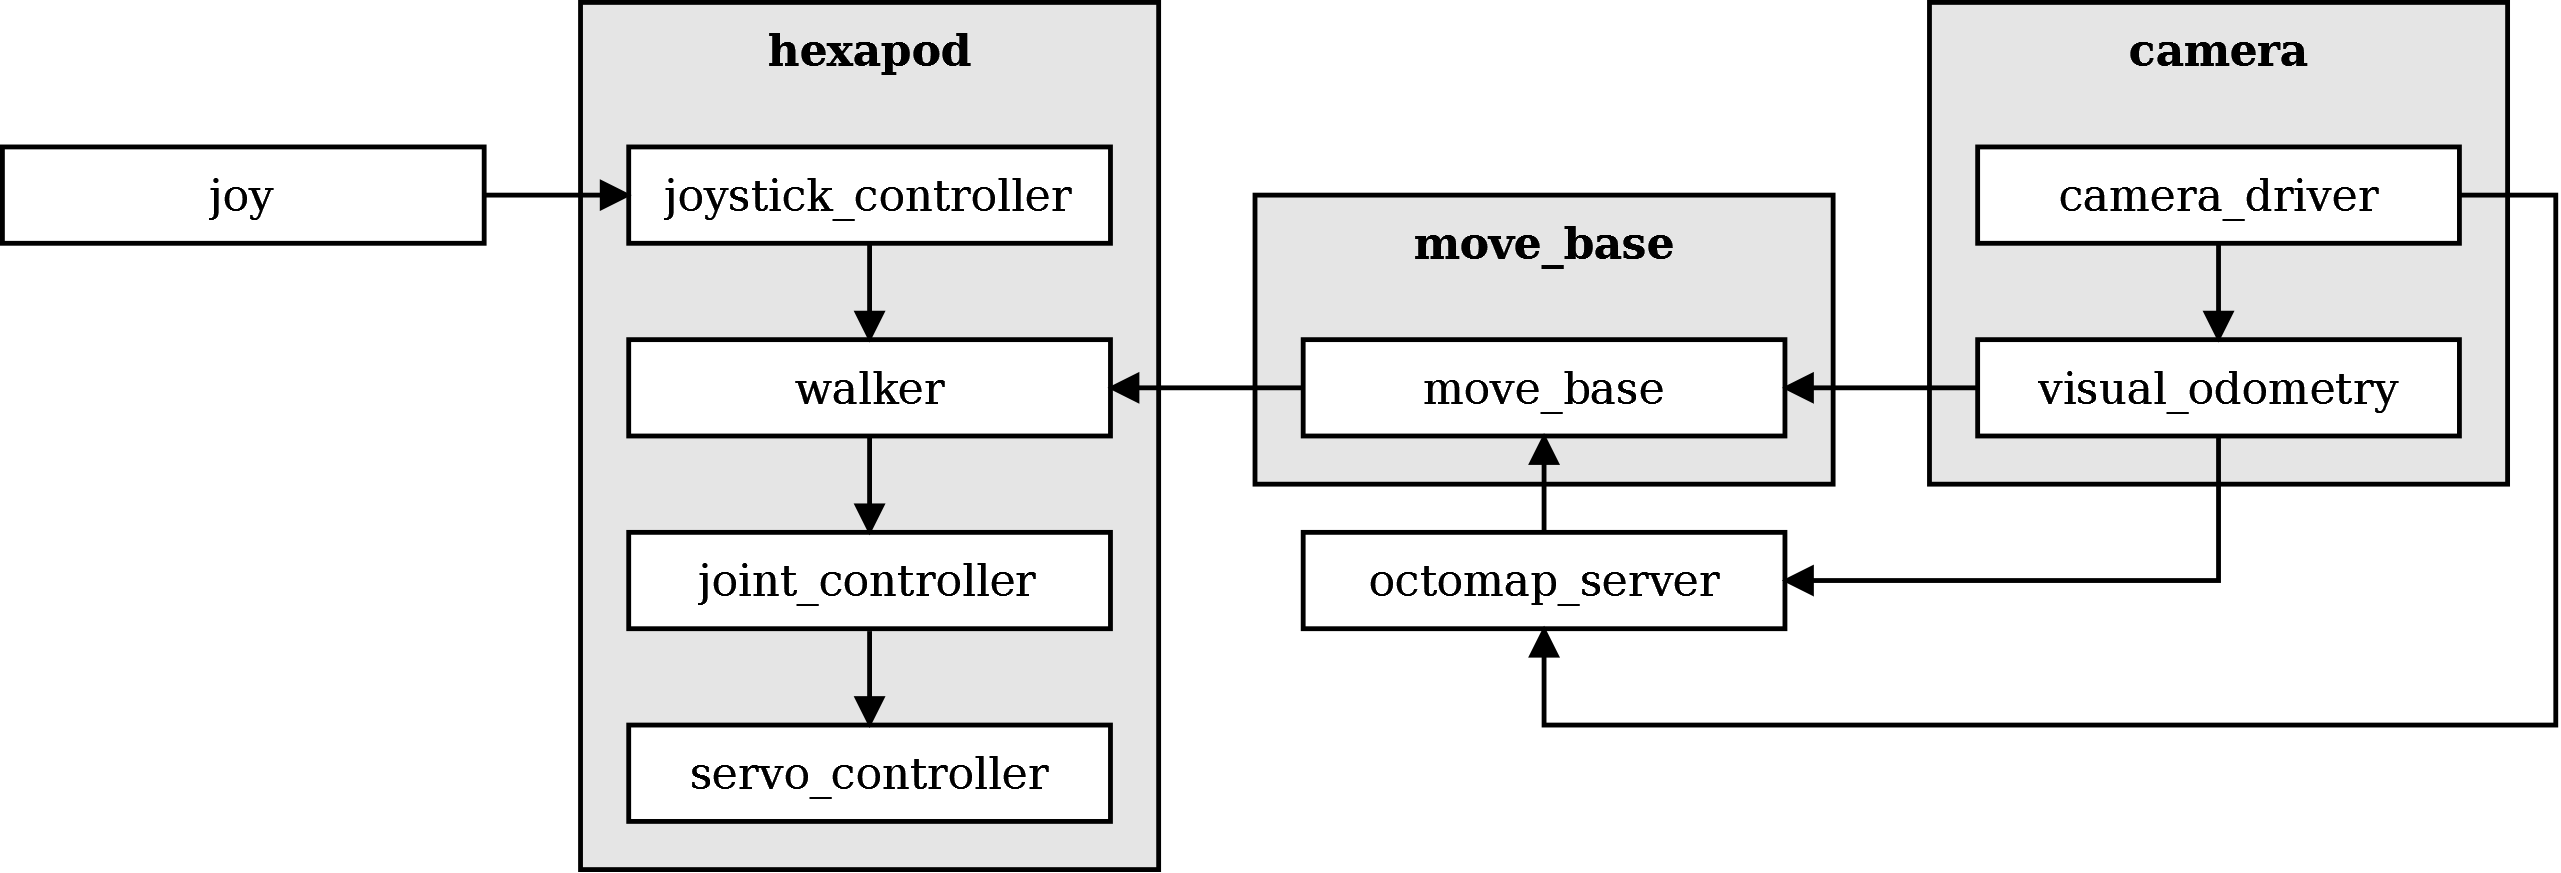
\includegraphics[width=16cm]{nodes.png}
    \caption{A simplified diagram showing an example of node relations, modelled after the implemented robot system. White boxes represent particular nodes, while the grey boxes surrounding them represent a namespace in which they exist. Arrows between nodes indicate a communication flow.}
    \label{fig:rviz}
\end{figure}

As intraprocess communication can be somewhat costly in terms of performance, ROS provides a means for running multiple nodes in the same process via \emph{nodelets} \cite{ros_wiki_nodelet}. This allows messages to be passed in a zero copy manner, as pointers to memory locations where messages are stored can be shared directly. Nodes must be modified to support this behaviour, however, as they must export some class that can be dynamically loaded by a \emph{nodelet manager}. This feature is used extensively when real-time performance is required such as with computer vision related tasks, for example.

\subsection{Topics \& Services}
Node communication is done through \emph{topics} in a one-to-many fashion \cite{ros_paper}. Broadcasting is done asynchronously, such that the broadcasting node can continue operating without regard as to which nodes receive the message. Any other node can then subscribe to that particular topic, receiving messages through a callback for processing. Each topic has a given resource name which is used to uniquely identify that topic.

A topic is defined with a given \emph{message} type through \emph{msg} files. Messages are simple data structures consisting of a number of typed data fields. Each data field has a unique name, and can be of a number of built-in primitive types, as well as other arbitrarily nested data structures such as arrays and even other messages. A simple example of this would be the \texttt{Point} message from the \texttt{geometry\_msgs} package. This message consists of three \texttt{float64} fields named \texttt{x}, \texttt{y}, and \texttt{z} \cite{ros_api_point_msg}.

ROS also provides a \emph{request-response} style method of communication through \emph{services} \cite{ros_wiki_services}. In this case, a \emph{service} type is defined, in a format similar to topic messages, through \emph{srv} files. However, it differs in that two messages are defined in one file---one for the request and the other for the response. This communication method is synchronous, in that a requesting node will block until a response is given. 

\subsection{Resource Names}

Each resource in the system has a unique name, and can be placed into a namespace. This gives each resource a unique \emph{graph resource name} which can be used to identify this resource elsewhere throughout the system. As the name suggests, the layout of a ROS system can be thought of as a graph or tree. Some examples of \emph{graph resource names} are shown below.

\begin{figure}[!h]
    \centering
    \begin{tabular}{  l l  }
        \textbf{Path} & \textbf{Description} \\
        \hline
        \texttt{/} & the global namespace \\
        \texttt{/hexapod/} & the \texttt{hexapod} namespace \\
        \texttt{/hexapod/servo\_controller} & a \texttt{servo\_controller} node \\
    \end{tabular}
\end{figure}

\subsection{Packages}
A collection of nodes providing a particular set of functionalities (e.g., path planning for autonomous navigation), can be grouped and distributed as \emph{packages} \cite{ros_paper}. This can be used to divide nodes in a system into logical subsystems. By developing nodes and packages in a generic way, they can also act as a means for providing drop-in functionality.

Users are encouraged to share and distribute any developments they make by hosting repositories of their code, preferably on \emph{GitHub} \cite{ros_wiki_getinvolved}. Contributors can then request that their repository be listed on a package index on the ROS website \cite{ros_wiki_getinvolved}. This aspect is a particular advantage of ROS, as there is a wide array of packages available for usage. Additionally, as ROS provides a number of common data types used in robotics, packages from different vendors can interact with one another with relative ease.

\subsection{Standard Packages \& Utilities}
The standard ROS distribution contains a number of standard packages and utilities. These provide a number of essential features that streamline the entire development process. A number of these are particularly useful for use with our robot control system.

\subsubsection{roslaunch: Programatically Start Nodes}
While nodes can launched manually, ROS provides a means for large sets of nodes programmatically via \emph{roslaunch} \cite{ros_paper, ros_wiki_roslaunch}. This tool allows developers to specify a set of nodes to be ran, along with a number of parameters, in XML configuration files (``launch files'' in ROS terminology). \emph{roslaunch} provides a number of useful features.

A key feature is the ability to specify which namespace a particular set of nodes is in. This allows multiple nodes of the same type to be launched without conflict. Any topic used by a node can also be remapped to one more appropriate. This means that nodes can be built generically, assuming that their topics will be remapped to fulfil some specific purpose. An example of this is the \texttt{depthimage\_to\_laserscan} node, which converts a depth image into a format usable by nodes expecting laser scan data. This node expects the depth image to be transmitted on \texttt{/image}, assuming that this will be remapped to the actual depth image.

Launch files can also include other launch files. Generally, a package will provide a launch configuration that starts all the necessary nodes to provide dealing with this package. This can be used to create a ``master'' configuration that launches a number of necessary subsystems.

\subsubsection{rviz: Visualising Sensor Data}

In addition to providing autonomous behaviour, it is often necessary that a control system must be able to provide some useful visualisations to the user operating the system. This can be much more helpful for gaining an understanding of what data the system is receiving, versus trawling through text logs alone. Rather than having to develop new visualisation software for every robot system, ROS provides a generic means for achieving this via \emph{rviz} \cite{ros_wiki_rviz}.

\begin{figure}[!h]
    \centering
    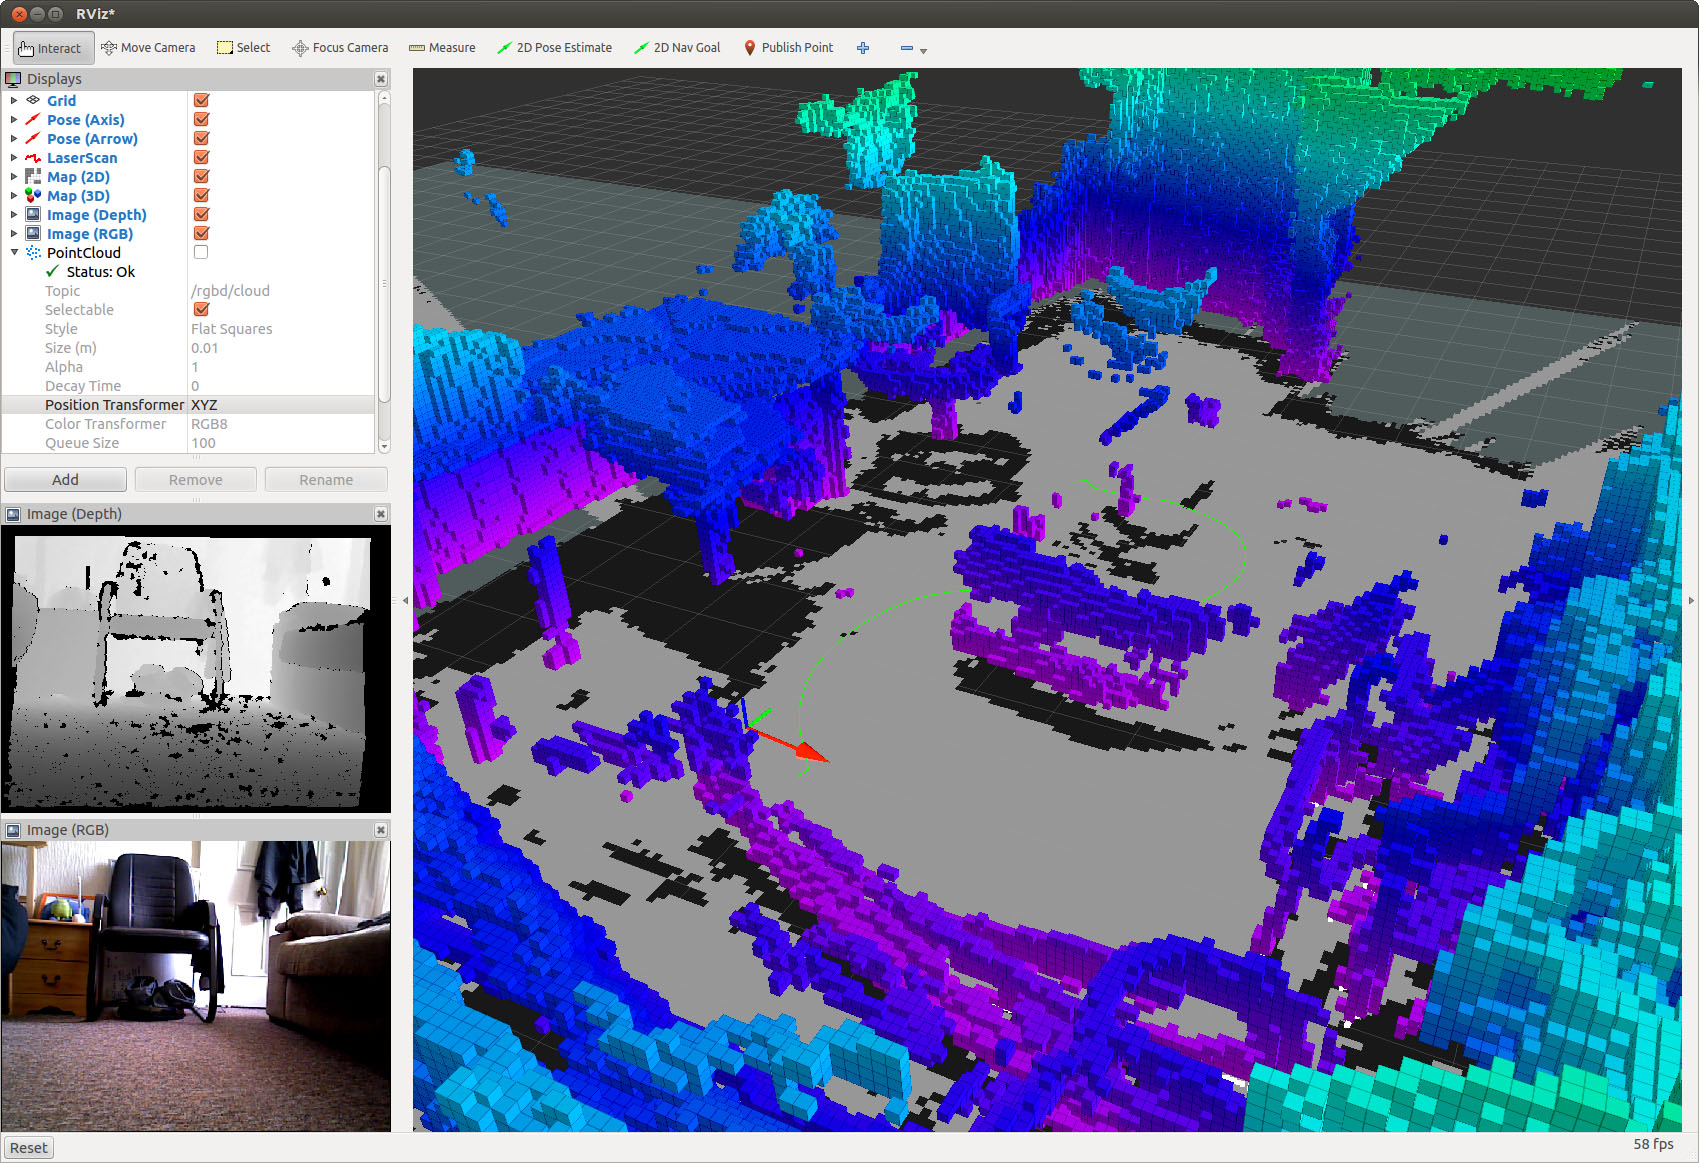
\includegraphics[width=15cm]{rviz1.jpg}
    \caption{An example configuration of RViz, specifically in the configuration used for the robot control system. The two image feeds from the camera can be seen on the left hand side, along with the configuration window for each visualisation. The main window shows the space in which the robot is operating, where a number of visualisations show the positioning and mapping facilities of the system. The green line, in particular, represents the current navigational path that the robot will follow.}
    \label{fig:rviz}
\end{figure}

\emph{rviz} is a highly configurable program, primarily for displaying visualising data from topics in the system. It can be considered the hub of interactivity for the robot control system, allowing a user to control and understand the underlying system. Visualisations are made possible through a plugin system, a number of which are distributed with the package. These plugins provide visualisations for a number of common messages \cite{ros_wiki_rviz_datatypes}, examples of which are shown in \autoref{fig:rviz}. A major advantage of this plugin concept is that new visualisations can be developed an integrated with \emph{rviz} easily, without having to modify the core of the program itself. This may be necessary if a control system implements some new type of message, for example. In particular, many community-provided packages implement new visualisations for their custom messages.

Additionally, it is possible to interact with the control system through \emph{rviz} through \emph{interactive markers} \cite{ros_wiki_rviz_intmark}. A user is able to move or rotate these markers on-screen, depending on the configuration, which can be used to control a corresponding robot limb, for example. The same markers can also be used to set navigational waypoints which a robot can then follow. Internally, marker data is transmitted and received through the usual topic system.

\subsubsection{tf: Transforming Between Various Coordinate Frames}
A common problem in robotics is the need to transform between different coordinate frames. For example, a number of laser rangefinders may be placed in varying positions around the the base of a robot. The incoming range data from a rangefinders will be relative to its origin. Should it be necessary to find the distance from the base of the robot to a nearby wall in sight of the rangefinder, for example, some arithmetic must be performed to calculate the distance, based on the physical offsets between the base and the rangefinder. Rather than performing these calculations manually each time, ROS provides a standard solution for achieving this through the \emph{tf} package \cite{ros_wiki_tf}. An annotated example of these concepts is shown in \autoref{fig:tf}.

\begin{figure}[!h]
    \centering
    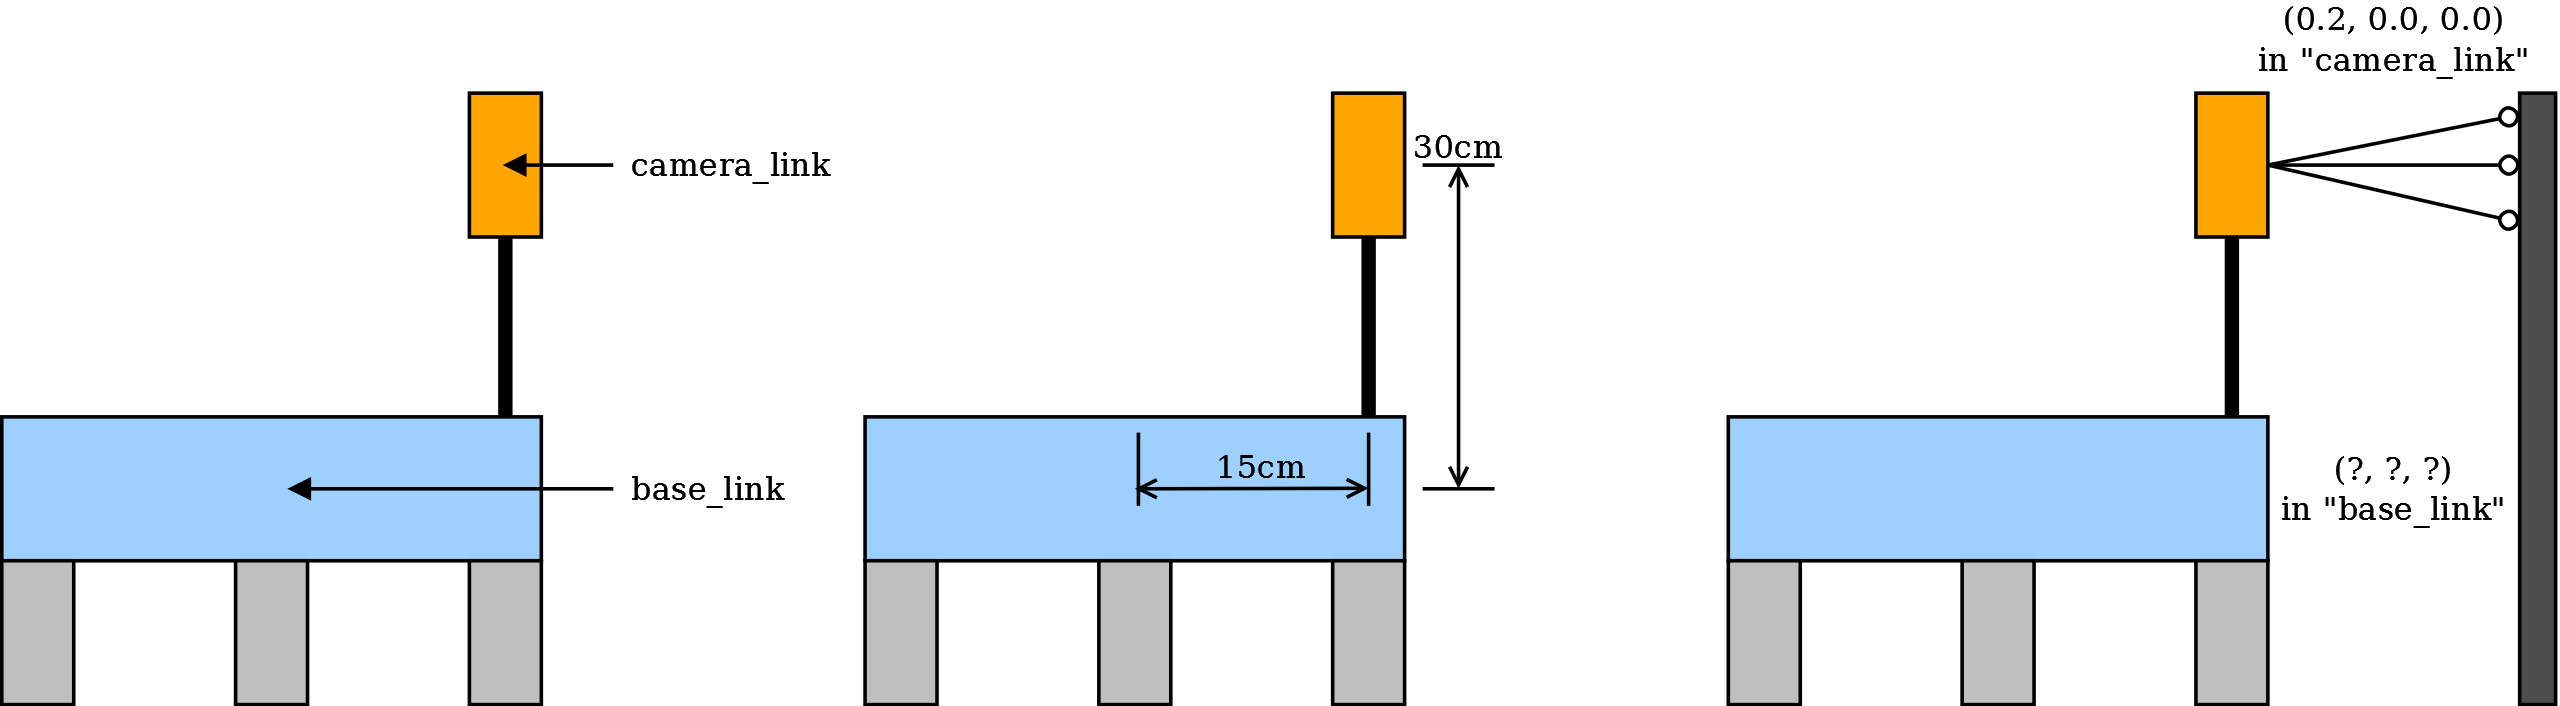
\includegraphics[width=17cm]{tf2.png}
    \caption{A diagram showing the necessity for some sort of transformation system, modelled after the robot. In the first picture, the two transformation links for this robot are shown. In the second picture, the distances between the origins of the two transformation links are shown. Specifically, it can be said that \texttt{camera\_link} is positioned at an offset of (0.15, 0.30, 0) meters relative to \texttt{base\_link}. The inverse of this is also true, in that \texttt{base\_link} is positioned at an offset of (-0.15, -0.30, 0) meters relative to \texttt{camera\_link}. In the third picture, points detected on a wall at a distance of (0.2, 0, 0) meters relative to the camera are shown. By applying the transformation offsets between \texttt{camera\_link} and \texttt{base\_link}, it is possible to calculate the distance of the points relative to base of the robot. Through simple arithmetic, the points can be calculated to show that the points are at a position of (0.35, 0.3, 0) meters relative to the base of the robot.}
    \label{fig:tf}
\end{figure}

The relations between different coordinate frames and their transformations are represented in a tree-like hierarchy, where each node corresponds to a particular coordinate frame. A fixed frame is used as the root of this node, representing a coordinate frame which the rest can relate to. This fixed can represent the environment around a robot, for example. By traversing through this tree, it is possible to calculate positions in one coordinate frame relative to another. An example transform tree is shown in \autoref{fig:tf_tree}.

\begin{figure}[!h]
    \centering
    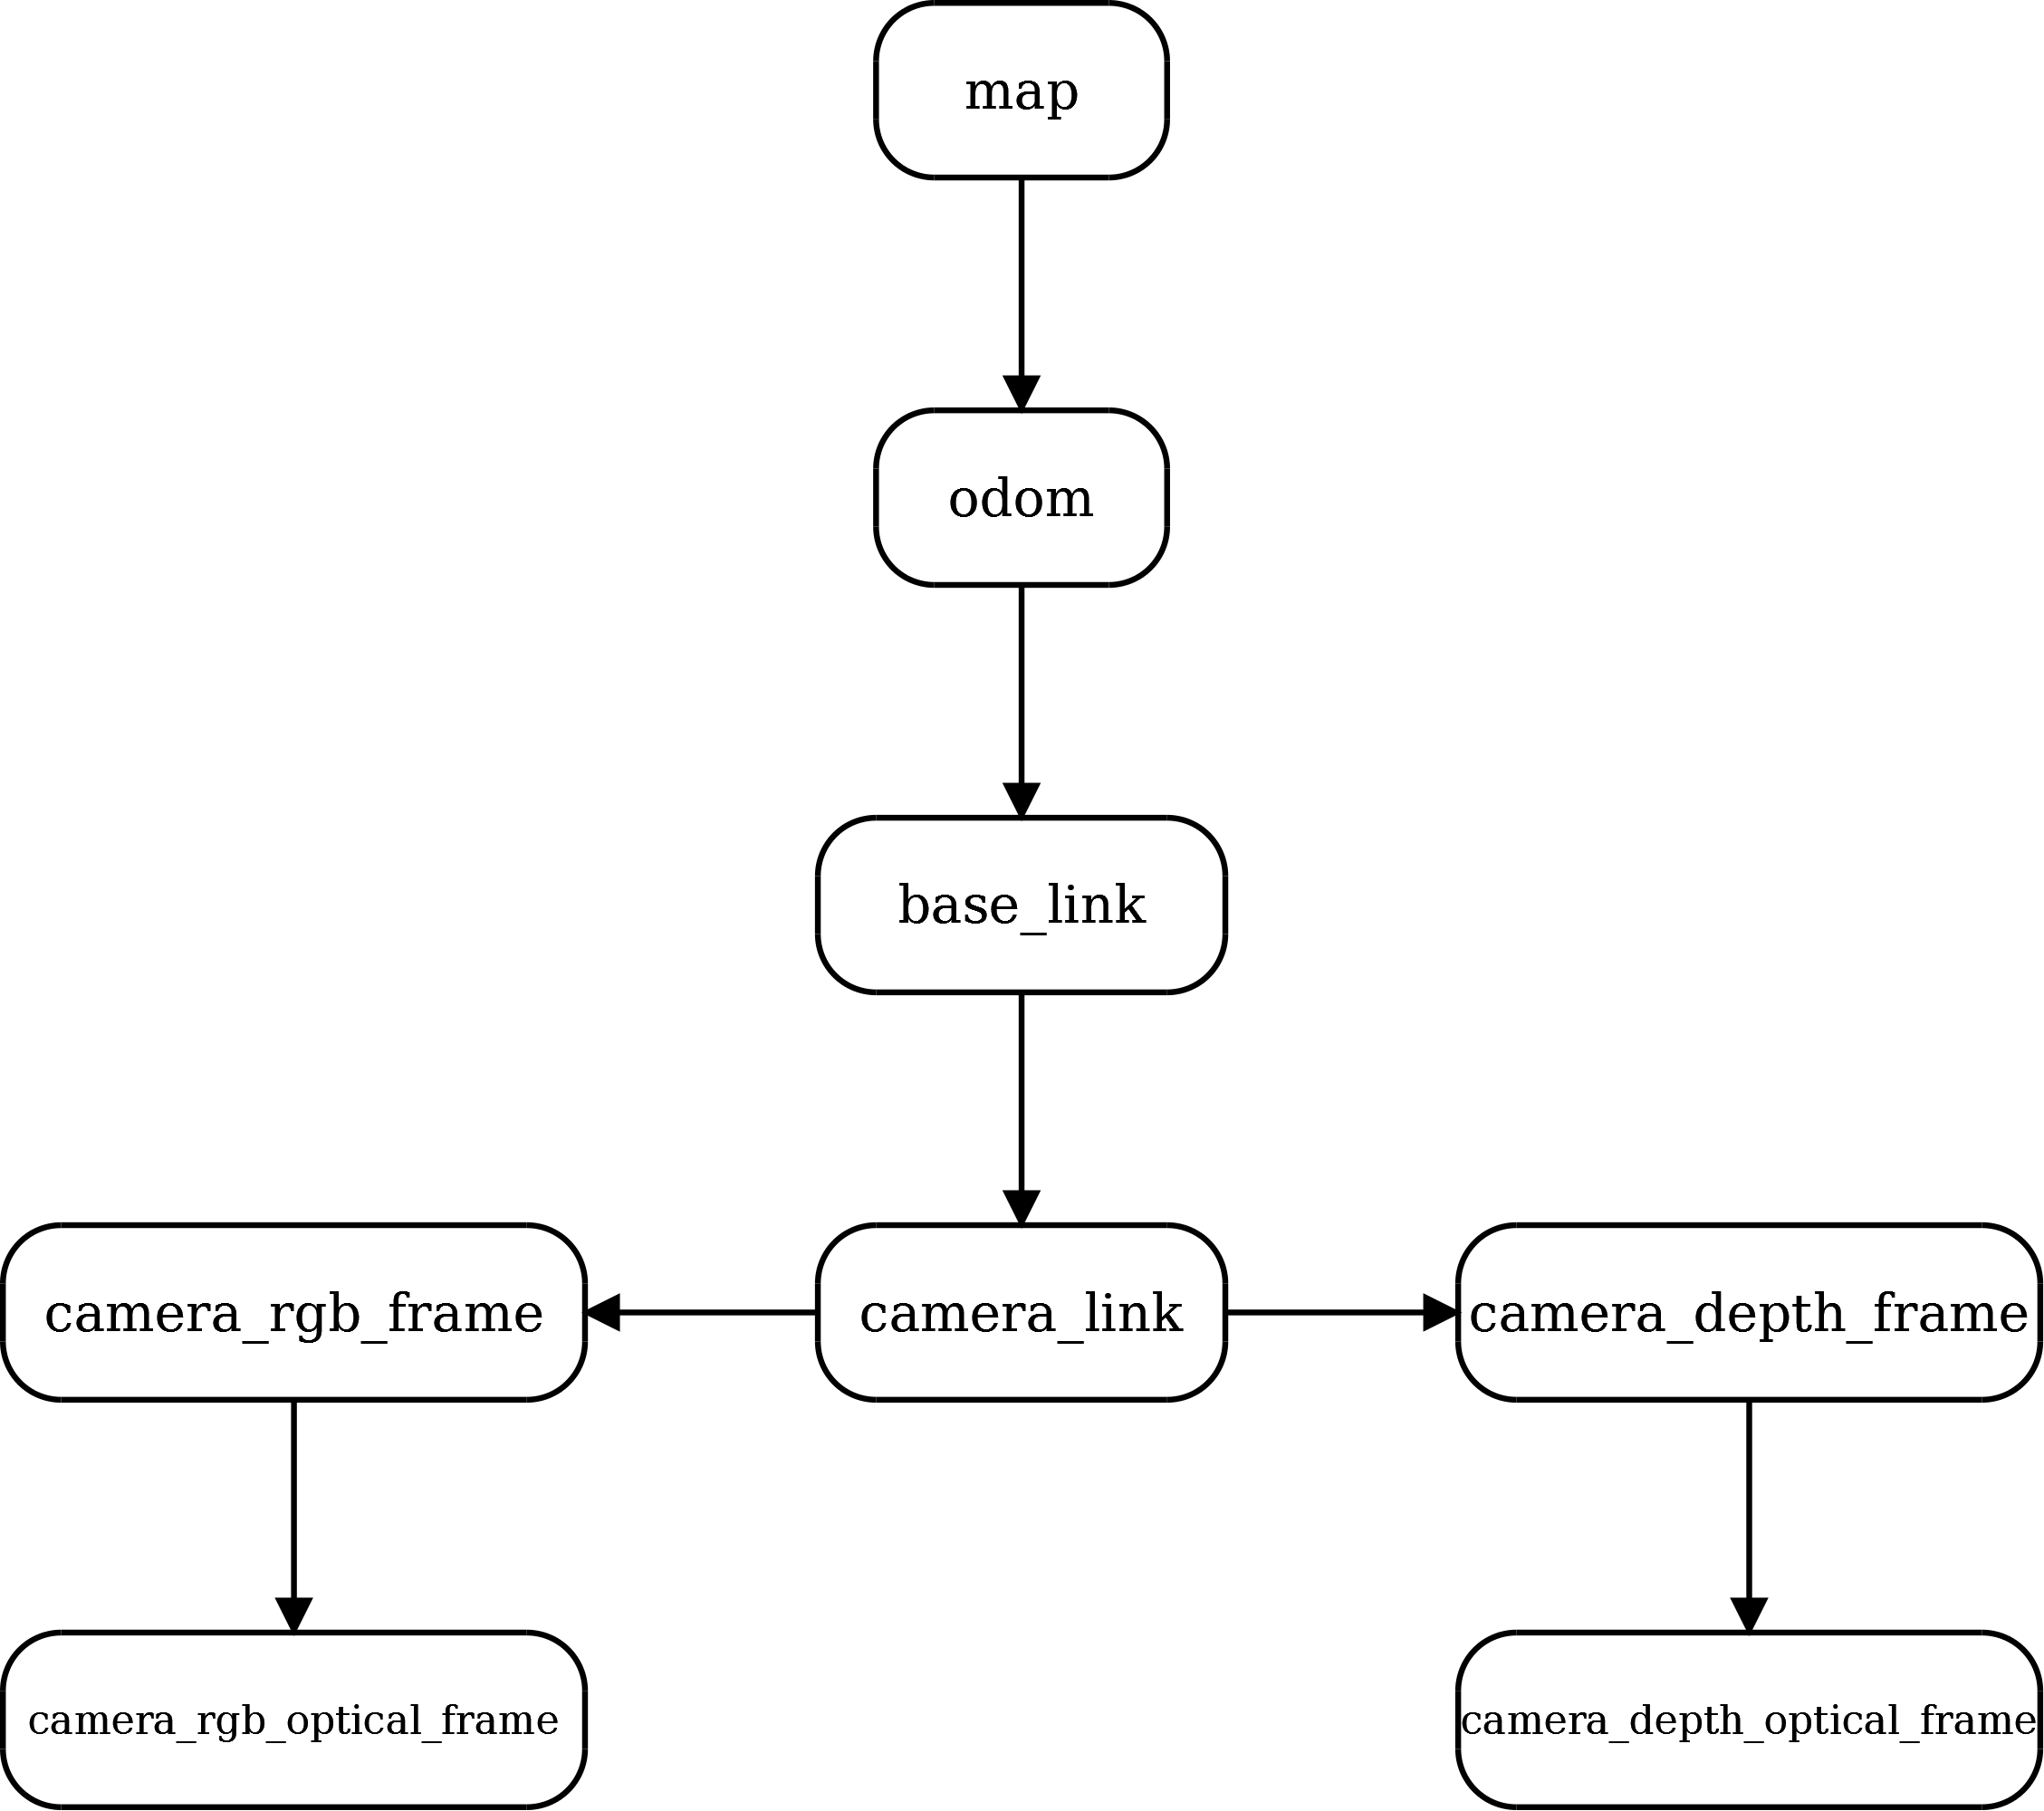
\includegraphics[width=10cm]{tf.png}
    \caption{An simplified diagram of a transform tree, modelled after the implemented robot control system. The boxes represent a transforms, while arrows between these boxes indicate a transform relation. Each transform provides its position and rotation in space, relative to the previous transform. For example, it is possible to get the position of the RGB-D camera relative to the environment by requesting a transform between \texttt{camera\_link} and \texttt{map}. The tf system will compute the resulting position based on the supplied transforms, working backwards through the hierarchy as necessary.}
    \label{fig:tf_tree}
\end{figure}

The \emph{tf} package has a variety of useful features. Transform positions are cached throughout run-time such that it is possible to request positions at times in the past. Additionally, a number of nodes are available in the \emph{tf} package that can publish static transforms between coordinate frames. In the example show in \autoref{fig:tf}, one would use these nodes to publish the offsets between base of the robot and the camera.

%%%%%%%%%%%%%%%%%%%%%%%%%%%%%%%%%%%%%%%%%%%%%%%%%%%%%%%%%%%%%%%%%%%%%%%%%%%%%%%%%%%%%%%%%%%%%%%%%%%%

\section{Hardware}

The robotic hardware used in this project is relatively straightforward, consisting of a number of off-the-shelf components. The robot is a hexapod-type, in that it has six limbs. Each limb has three joints at which it can rotate, as shown in \autoref{fig:hexapod_dof}, giving three degrees-of-freedom per limb. 

\begin{figure}[!h]
    \centering
    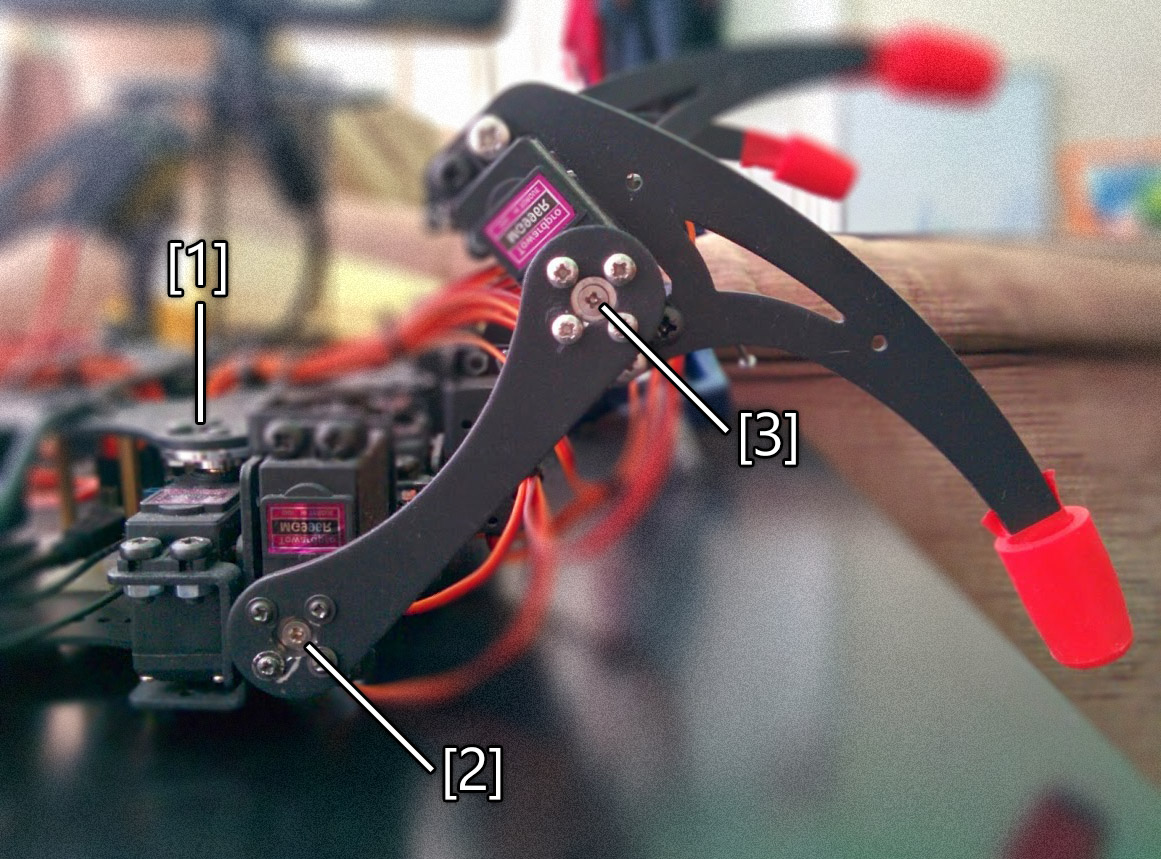
\includegraphics[width=12cm]{hexapod_joints}
    \caption{This annotated photograph shows the three degrees-of-freedom available to each limb on the robot. Joint 1 provides horizontal rotation to the leg, allowing the robot to push itself forward. Joints 2 and 3 provide vertical rotation, which can be used to adjust the robots height, as well as being used for locomotion in general.}
    \label{fig:hexapod_dof}
\end{figure}

In its current state, the robot has no wireless capability and, thusly, operates in a tethered manner. A bundle of cables protruding from the rear end of the unit connects the on-board hardware to a nearby power source and computer.

\subsection{Servos \& Servo Controller}
Each joint piece is attached to the shaft of a servomechanism (servo) to facilitate rotation. Each servo is controlled by a \emph{pulse-width modulated} (PWM) signal supplied by the controller, such that the angle of the servo can be controlled. Servos operate using a feedback-loop system such that the current of a motor is controlled, rotating the shaft to the desired position. Rotational range and speed of servos vary depending on model, but in this case the servos allow for a total rotational range of 180\textdegree.

The servos are controlled by an off-the-shelf servo controller board. This board, in particular, expects text-based control commands over serial, either via direct TTL or emulated over an on-board USB to TTL converter \cite{torobot_manual}. A number of commands are supported, allowing control of the position of both single and groups of servos. Additionally, a set of movements can be programmed and issues with a single command \cite{torobot_manual}. Power is also distrusted to the servos via this board.

\subsubsection{Protocol}

Commands are issued using an ASCII-based protocol via serial communication. While the servo controller supports a number of commands, only the command which rotates an individual servo is necessary. This allows for more flexibility in terms of when the rotation begins, as all servos mentioned in a group command will begin rotation at the same time.

\begin{figure}[!h]
    \centering
    \texttt{\#\(n\)\#P\(a\)T\(t\)}
\end{figure}

A rotation command is issued by sending a string in the format shown above, specifying the particular servo number ($1 \leq n \leq 32$), the target position ($1500 \leq a \leq 2500$), and the time over which the rotation should occur ($100 \leq t \leq 9999$) in milliseconds. The command is ended by a carriage return followed by a new line character. A working example is shown below, where we rotate the servo at index 1 to 90\textdegree{} over 250ms.

\begin{figure}[!h]
    \centering
    \texttt{\#1\#P2000T250}
\end{figure}

It should be noted that the parameter for the target position is actually the pulse-width duration (in milliseconds) that is sent to the servo, rather than an actual angle. Duration ranges can very per manufacturer, however there is a common standard such that 1.5\textmu s corresponds to 0\textdegree{} and 2.5\textmu s correspond to 180\textdegree. These are the minimum and maximum possible values for this controller. 

\subsection{RGB-D Camera}
The primary sensor in the system is an \emph{ASUS Xtion Pro Live} RGB-D camera, which is very similar to the \emph{Microsoft Kinect}. The key functionality of this camera is that it provides a depth data feed, giving a range of values indicating the distances to the objects in front of it.

\begin{figure}[!h]
    \centering
    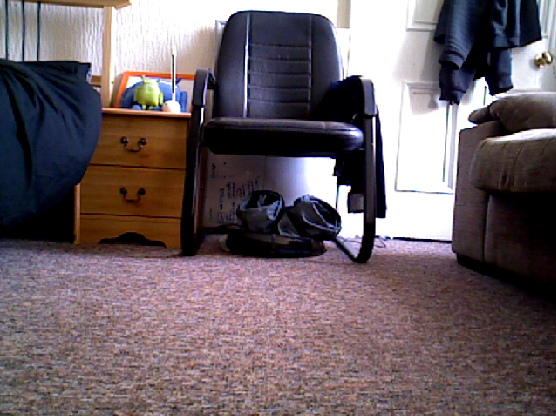
\includegraphics[width=8cm]{rgbd_rgb2.jpg}
    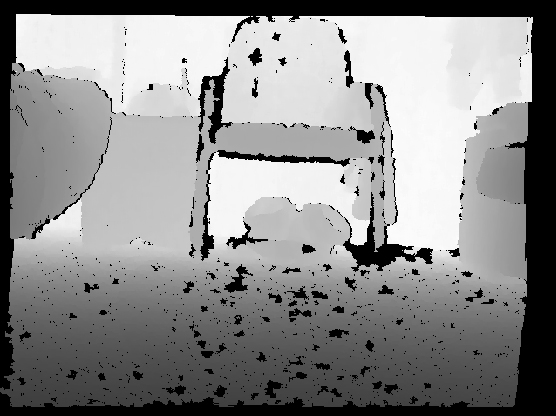
\includegraphics[width=8cm]{rgbd_depth2.jpg}
    \caption{Example imagery from the RGB-D camera mounted on top of the robot, as given by the \texttt{openni2\_camera} package. The image on the left shows the RGB output from the camera. The image on the right shows the depth output interpreted as a monochrome image.}
    \label{fig:rgbd_images1}
\end{figure}

The advantages this particular sensor provides over the \emph{Kinect} is mostly physical, specifically weight and footprint. The \emph{Kinect} has a motorized base which allows the device to be tilted upwards and downwards through software, in comparison to the \emph{Xtion} which has a simple hinge that can be rotated by hand. This feature is unnecessary in this use case and adds a significant amount of weight. Additionally, the \emph{Kinect} is intended to be a consumer device and, thus, has a much striking product design. However, this striking design comes at a cost of making the device much larger in general, which is somewhat troubling when it must be placed on an already space-starved robot base.

\subsubsection{OpenNI}
Should one which to develop for the \emph{Xtion} in general, they must use the \emph{OpenNI} framework. \emph{OpenNI} is a ``standard framework for 3D sensing'' \cite{openni_site}.

In particular, the \emph{Xtion} requires the use of \emph{OpenNI2}

%%%%%%%%%%%%%%%%%%%%%%%%%%%%%%%%%%%%%%%%%%%%%%%%%%%%%%%%%%%%%%%%%%%%%%%%%%%%%%%%%%%%%%%%%%%%%%%%%%%%

\section{Existing Examples}